\documentclass[conference]{IEEEtran}
\usepackage{amsmath,amssymb,graphicx,booktabs,multirow,tabularx,xcolor,url}
\usepackage[caption=false,font=footnotesize]{subfig}
\graphicspath{{figures/}}
\definecolor{tbdred}{RGB}{190,0,0}
\newcommand{\datasetrows}{%
Moon & 20 & 0.25--0.25 & 0.32072 & Chandrayaan-2 OHRC / Roboflow \\
Mars & 60 & 5--10.2 (59/60 assumed) & 273.28 & Roboflow mixed-source Mars set \\
}

\newcommand{\detectionrows}{%
Moon (v1 Hough) & 626 & 399 / 217 / 10 & 48 / 391 / 130 / 57 \\
Mars (v2 Ellipse) & 1145 & 0 / 0 / 1145 & 21 / 399 / 502 / 223 \\
}

\newcommand{\validationrows}{%
Moon v1 Hough & 0.179 & 0.086 & 0.116 & 0.633 \\
Mars v1 Hough & 0.062 & 0.075 & 0.068 & 0.566 \\
Mars v2 Ellipse & 0.070 & 0.093 & 0.080 & 0.632 \\
}

\newcommand{\depthrows}{%
Moon & 626 & 1.35 & 0.148 & 0.0\% \\
Mars & 1145 & 59.10\textsuperscript{*} & 0.171 & 100.0\% \\
}

\newcommand{\missionrows}{%
Moon & 21.00 & 21.90 & 20.25 & 8.2\% & 0 / 0 & 1.82 \\
Mars\textsuperscript{*} & 590.00 & 625.42 & 580.45 & 7.7\% & 0 / 0 & 9.41 \\
}

\begin{document}
\title{Explainable Classical Computer Vision for Lunar and Martian Crater Detection, Physical Characterization, and Mission Planning}
\author{\IEEEauthorblockN{[Author Names]}\IEEEauthorblockA{SVKM's NMIMS Mukesh Patel School of Technology Management and Engineering\\\texttt{[emails]}}}
\maketitle

\begin{abstract}
Crater morphology supports planetary surface interpretation and is directly relevant to local hazard awareness, yet a crater outline alone is not enough to communicate how an image-derived measurement or route was produced. This paper describes an explainable classical computer-vision application that connects crater detection, physical characterization, and a crater-aware mission-planning demonstration for lunar and Martian image tiles. The implementation uses median filtering, CLAHE, Canny edges, Otsu shadow segmentation, and a Hough-circle detector for the Moon; Mars uses a separate ellipse-fitting detector with morphology-proposed candidates and edge-coverage filtering. Detected geometry is scaled with the tile resolution, then used to estimate shadow depth, depth-to-diameter ratio, and a heuristic freshness/degradation class. A crater cost map and eight-connected A* search identify a high-clearance touchdown candidate and a route to a selected crater rim. We ran the current repository pipeline over 20 lunar and 60 Mars tiles and evaluated against held-out YOLO labels using greedy one-to-one box matching at IoU 0.5. The reported results are generated from these runs and retain the detectors' limitations: Mars scale is assumed for most tiles, depth estimates are low confidence on Mars, and the planner considers craters only. The contribution is an integrated, inspectable workflow rather than a new detection algorithm.
\end{abstract}
\begin{IEEEkeywords}
planetary image analysis, crater detection, classical computer vision, ellipse fitting, Hough transform, hazard mapping, A* search
\end{IEEEkeywords}

\section{Introduction}
Impact craters are useful landmarks and records of surface modification. Their population and morphology inform geological interpretation, while local crater geometry can help identify hazards around a candidate landing site. Operational terrain-relative navigation systems use richer maps and onboard sensing: NASA's Jezero hazard map, for example, depicts landing hazards and safer areas for Perseverance's landing process~\cite{jplJezero}. ISRO also documented a crater encountered during Pragyan's traverse on 27 August 2023~\cite{isroPragyan}. These examples motivate a small-scale project that makes image-derived crater and route decisions visible to a user.

This work addresses a practical educational engineering problem: how to connect classical image processing outputs to physical measurements and an interpretable route-planning display on two planetary datasets. It is not an operational navigation system. The application has separate detectors because the Moon tiles are treated as approximately circular at their image scale, whereas the Mars image set includes more varied appearances and elongated projected rims.

The contributions are:
\begin{itemize}
\item An end-to-end interface connecting edge/shadow processing, crater candidates, geometric and physical descriptors, and visual overlays.
\item A planet-specific implementation using Hough circles for lunar tiles and an ellipse-fitting detector for Mars tiles, with intermediate imagery exposed for inspection.
\item A crater-only touchdown and rover-route demonstration using a cost grid, distance transform, and A* search, accompanied by held-out box-matching measurements.
\end{itemize}

Fig.~\ref{fig:system} summarizes the application flow. All performance tables and plots in this paper are generated from current project-code runs and the dataset labels; exact dataset counts and output values are presented in Tables~\ref{tab:data}--\ref{tab:mission}.

\begin{figure*}[!t]
\centering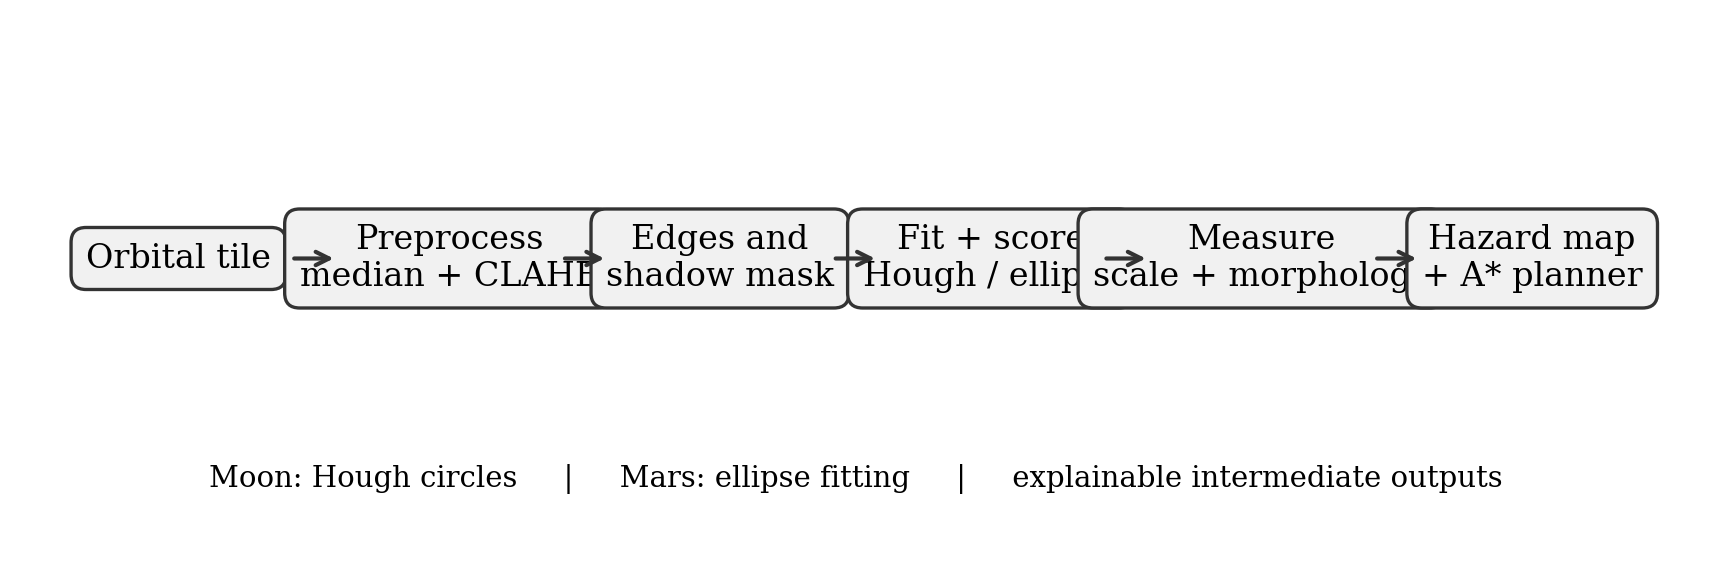
\includegraphics[width=.98\textwidth]{system_diagram.png}
\caption{System block diagram. The lunar Hough and Mars ellipse branches feed common measurement and crater-based planning components.}
\label{fig:system}
\end{figure*}

\section{Related Work}
Classical crater detection includes shape-and-texture candidate filtering and edge-based geometric fitting. Bandeira \emph{et al.} studied sub-kilometer crater detection using shape and texture features~\cite{bandeira2012}; Kim and collaborators described a Mars crater workflow combining image and terrain data and ellipse-oriented analysis~\cite{kim2004}. Hough transforms have also been applied to crater detection and counting, with preprocessing and edge quality affecting performance~\cite{galloway2014}. These studies provide context for this project's detector choices; they do not imply that the application reproduces their full methods.

Global crater inventories support comparative planetary science, including a global Mars impact-crater database~\cite{robbinsHynek2012} and a global lunar crater database~\cite{robbins2019}. Crater depth-to-diameter ratios are influenced by crater size, target material, and degradation, so a single ratio is not a unique age or material indicator~\cite{stopar2017}. Chronology uses crater populations with calibrated context, not isolated image-tile counts~\cite{ivanov2001}. Recent Chandrayaan-2 crater work has also explored deep convolutional networks on TMC-2 imagery~\cite{sinha2024}; it is a distinct sensor/data and modeling setting from the classical pipeline here.

\section{Datasets}
The lunar set is the Roboflow YOLO export identified as Chandrayaan-2 OHRC imagery; OHRC is the orbiter's high-resolution camera instrument~\cite{ohrc2020}. The project assigns a nominal ground sampling distance of 0.25~m/pixel. The Mars set is a separate Roboflow export whose filenames and source descriptions indicate a mixed collection; scale is stored per tile when calibrated and otherwise the application falls back to 5~m/pixel. The dataset metadata identify both exports as CC BY 4.0. Table~\ref{tab:data} reports observed tile counts and summed tile footprint areas from the actual image dimensions and configured scales. This sum does not remove possible overlap between tiles, and Mars footprint values inherit the fallback scale where uncalibrated.

\begin{table*}[!t]
\caption{Dataset summary generated from the image files and tile configuration. Area is the sum of tile footprints; overlap is not removed.}
\label{tab:data}
\centering\scriptsize
\begin{tabular}{lrrrl}
\toprule Planet & Tiles & Resolution (m/pixel) & Summed area (km$^2$) & Source \\
\midrule
\datasetrows
\bottomrule
\end{tabular}
\end{table*}

\section{Methodology}
\subsection{Image processing and detection}
For the common Moon path, BGR input is converted to grayscale, median-filtered with a $5\times5$ kernel, and enhanced using CLAHE (clip limit 2.0, $8\times8$ tiles)~\cite{zuiderveld1994,gonzalez2018}. Canny thresholds are set to 0.55 and 1.45 times the median enhanced intensity~\cite{canny1986}. Otsu thresholding produces an inverse binary shadow candidate image followed by $3\times3$ elliptical opening and closing~\cite{otsu1979}. The Hough gradient transform proposes circles~\cite{duda1972}; each is scored by Canny edge density in a narrow annulus around the rim, then duplicate centers are suppressed. Mars v2 instead uses mild width-scaled Gaussian smoothing, Canny edges, size-scaled elliptical morphological closing and contour proposals; fitted ellipses are filtered by axis ratio and 36-sector rim coverage. Its axis-aligned output box follows the fitted ellipse extents. The separate Mars v1 Hough mode is retained for the validation comparison. The Mars v2 implementation is inspired by candidate-region and ellipse-fitting literature, but is an empirical project implementation, not an exact reproduction of prior algorithms.

Table~\ref{tab:pipeline} maps each processing stage to the implementation actually run. In particular, Mars v2 skips CLAHE in its own candidate branch even though the common pipeline computes CLAHE intermediates for shared descriptors and display.

\begin{table}[!t]
\caption{Pipeline stages and implemented image-processing techniques.}
\label{tab:pipeline}
\centering\scriptsize
\begin{tabularx}{\columnwidth}{p{.23\columnwidth}p{.36\columnwidth}X}
\toprule Stage & Technique & Purpose \\
\midrule
Input cleanup & Grayscale, median $5\times5$ & Reduce speckle while retaining edges \\
Contrast & CLAHE, clip 2.0 & Local contrast for common image branch \\
Rim cues & Adaptive Canny & Candidate edge pixels \\
Shadow mask & Inverse Otsu; morphology & Expose dark basin regions \\
Moon fit & Gaussian blur; Hough circles & Circle centers and radii \\
Mars fit & Gaussian blur; closing, contours, ellipse fit; 36-sector edge coverage & Elliptical crater candidates \\
Scoring & Rim-edge score; NMS & Rank and suppress redundant fits \\
Measurement & Pixel scale, shadow heuristic, texture/rim score & Diameter, depth, $d/D$, freshness class \\
Planning & Raster cost layers; distance transform; A* & Touchdown and rover path \\
\bottomrule
\end{tabularx}
\end{table}

\subsection{Geometric and physical descriptors}
For a circular detection of pixel radius $r_{\mathrm{px}}$ and tile scale $s$ in m/pixel, diameter is
\begin{equation}
D_{\mathrm{m}}=2r_{\mathrm{px}}s.
\label{eq:diameter}
\end{equation}
Mars ellipse detections use the detector's geometric-mean semi-axis as the reported radius; axis-aligned boxes retain the major/minor geometry for display and evaluation. Diameters below 10~m are Small, 10--30~m Medium, and at least 30~m Large in the shared classifier. The Mars class counts therefore inherit assumed scales for most tiles.

The depth routine takes an intensity scanline through each detected center. It marks pixels below 0.70 times that scanline's mean intensity as shadow pixels. If their fraction is $q$, the estimated horizontal shadow length is $L_{\mathrm{px}}=2r_{\mathrm{px}}q$ and $L_{\mathrm{m}}=sL_{\mathrm{px}}$. With configured solar elevation $\theta$, the implemented estimate is
\begin{equation}
d_{\mathrm{m}}=L_{\mathrm{m}}\tan(\theta),\qquad (d/D)=d_{\mathrm{m}}/D_{\mathrm{m}}.
\label{eq:depth}
\end{equation}
This is a one-dimensional threshold heuristic, not a recovered terrain profile. Shadow-derived crater morphology has been studied with topographic and controlled measurement approaches~\cite{pike1984,stopar2017}; this image scanline estimate is much less constrained. The Mars results are flagged low confidence because the tiles can be shaded or color-composited and do not provide reliable cast-shadow geometry.

Freshness uses rim edge occupancy $R$ (mean Canny value in the radius $r\pm3$ band divided by 255) and a floor-uniformity term $U=1-\min(\sigma_{\mathrm{floor}}/60,1)$, where the floor region is a disk of radius $0.6r$ in the enhanced image. The implemented score is
\begin{equation}
F=0.6R+0.4U.
\label{eq:freshness}
\end{equation}
Thresholds $F>0.48$, $F>0.32$, and $F>0.18$ assign Fresh, Slightly Degraded, and Moderately Degraded, respectively; remaining detections are Heavily Degraded. This is a heuristic image score rather than a calibrated geomorphological age measure.

\subsection{Crater cost map and A* route}
The planner rasterizes the tile at cell size $c=\max(1,s)$ meters. For crater $i$, a conservative radius $r_i$ uses the detector radius or ellipse major semi-axis, whichever is larger; rover footprint radius is $r_v$. The rim expansion is $b_i=b_0+0.25r_i$, with default $b_0=1$~m. Crater interiors expanded by the rover radius are impassable. The annular rim region receives cost $50(1+F_i)$; the outer halo receives $5(1+0.5F_i)$; clear cells have unit cost. Overlaps retain the larger cost. The implementation also reserves a narrow tile-edge margin. Low-confidence detections are included as hazards.

Touchdown candidates are chosen from hazard-free cells using a Euclidean distance transform of crater keep-out regions. The maximum-clearance cell is recommended if its clearance exceeds lander footprint radius plus margin; otherwise that maximum is displayed as best available and explicitly marked insufficient. The default footprint radius is 2~m and the margin is 1~m.

The rover objective defaults to reaching a detected crater rim. A* uses eight-connected neighbors, orthogonal step length 1, diagonal length $\sqrt{2}$, and mean endpoint traversability cost~\cite{hart1968}. For edge $(u,v)$ and heading change $\Delta h$, the implemented accumulated cost is
\begin{equation}
g(v)=g(u)+\ell(u,v)\frac{C(u)+C(v)}{2}+\tau\frac{\Delta h}{4},
\label{eq:astar}
\end{equation}
where $\tau$ depends on the selected route policy. Diagonal corner-cutting between blocked cells is disallowed. This grid search is not a vehicle dynamics model.

\section{Implementation}
The application is written in Python and uses OpenCV for filtering, morphology, fitting, and raster operations~\cite{bradski2000}; NumPy for array calculations; Pandas for catalog displays; Matplotlib for plots; and Streamlit for the interface. The current code exposes intermediate grayscale, enhanced, edge, binary, annotation, depth, hazard, catalog, and mission-planner views. The research exports in \texttt{paper/exports/} were generated by \texttt{paper/scripts/run\_experiments.py}; \texttt{collect\_results.py} reads those CSV exports and writes the table bodies included here. The experiment scripts do not modify the application or detector source.

Fig.~\ref{fig:stages} presents real intermediate images from one lunar tile. Fig.~\ref{fig:annotations} compares the two detector annotations, and Fig.~\ref{fig:jezero} gives the requested named Mars example (Jezero) with the dataset boxes visible alongside detections. These images are generated from actual project images and outputs, not mock-ups.

\begin{figure*}[!t]
\centering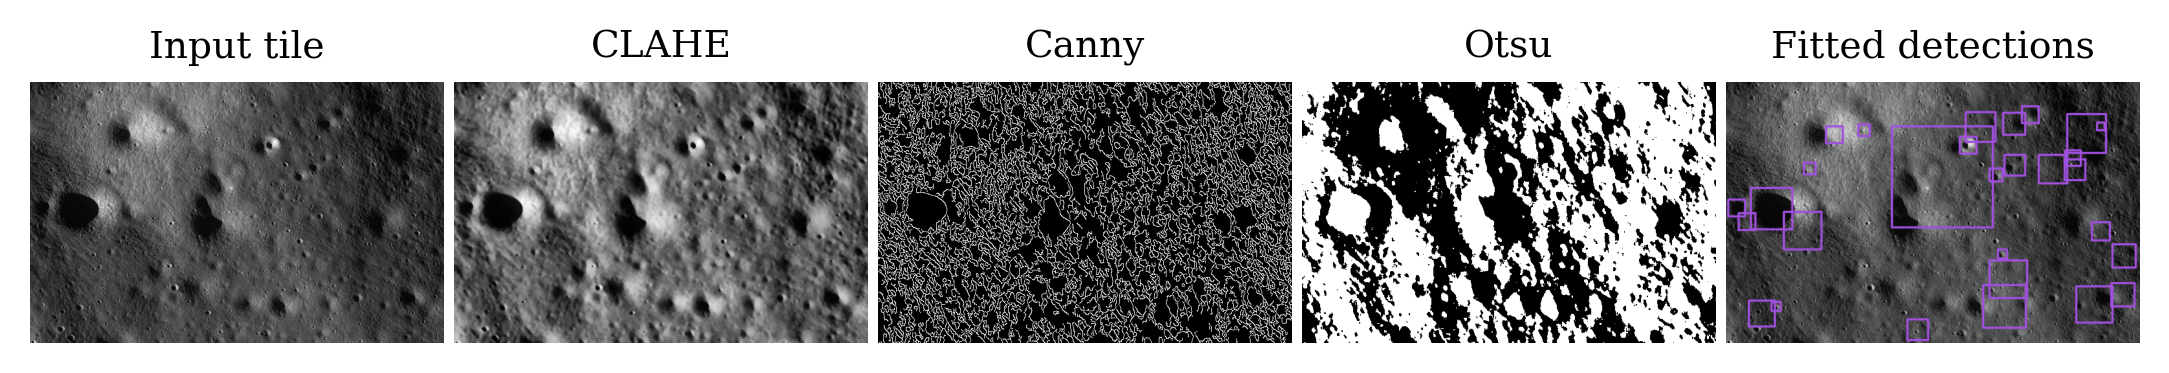
\includegraphics[width=.99\textwidth]{pipeline_stages.png}
\caption{Actual Moon tile through input, CLAHE, Canny, Otsu, and fitted-crater display.}
\label{fig:stages}
\end{figure*}
\begin{figure*}[!t]
\centering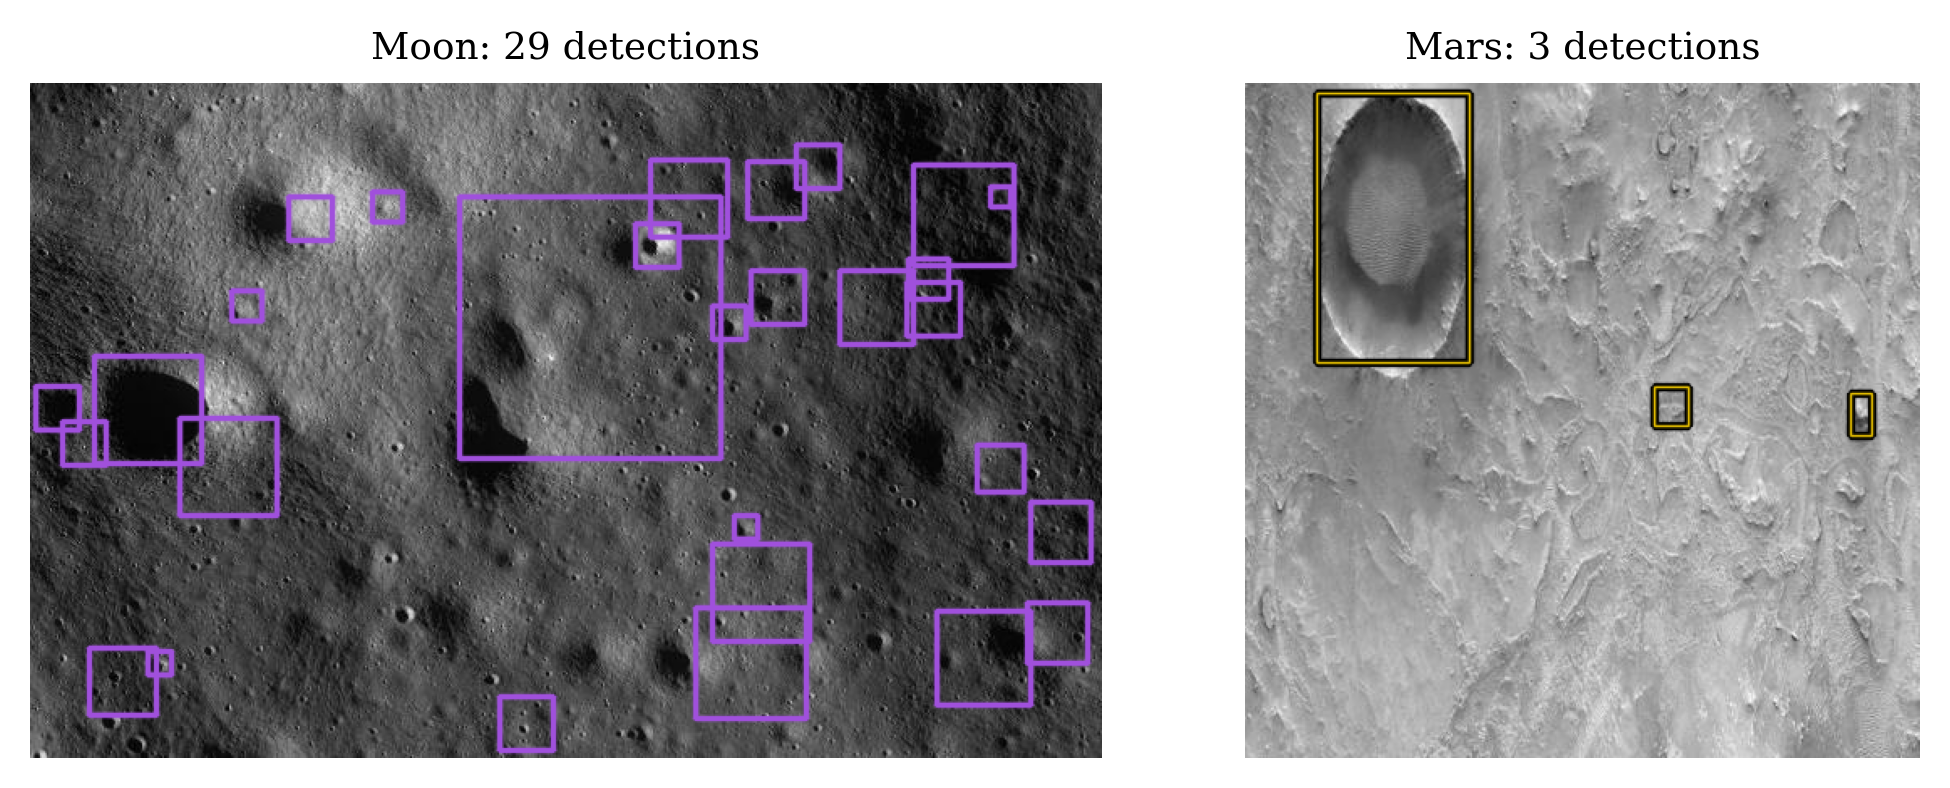
\includegraphics[width=.98\textwidth]{detections_planets.png}
\caption{Actual detector annotations: Moon in purple and Mars in yellow.}
\label{fig:annotations}
\end{figure*}
\begin{figure}[!t]
\centering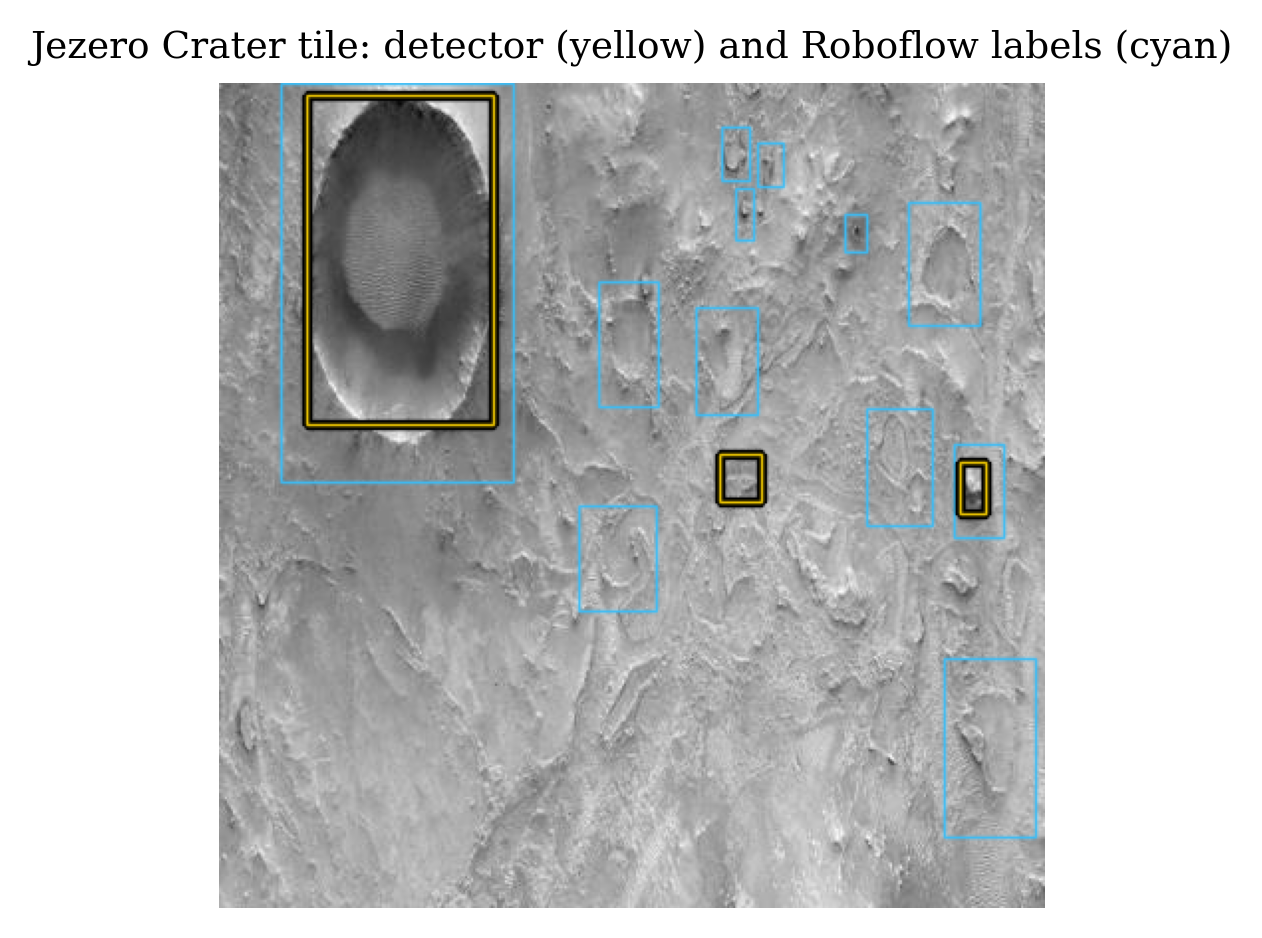
\includegraphics[width=\columnwidth]{jezero_labelled_example.png}
\caption{Jezero-labelled Mars tile. Yellow denotes v2 detections; cyan denotes exported Roboflow boxes.}
\label{fig:jezero}
\end{figure}

\section{Experiments and Results}
\subsection{Experimental protocol}
The dataset comprises the image tiles listed in Table~\ref{tab:data}; each tile is processed with planet defaults from \texttt{planets.py}. For the principal catalogs, Moon uses Hough v1 and Mars uses ellipse v2. Validation uses all four lunar \texttt{valid} tiles and the Mars \texttt{valid} and \texttt{test} splits (13 tiles total). Every YOLO box is retained. Predictions are converted to axis-aligned boxes and greedily matched one-to-one by descending IoU, with a match accepted at IoU $\geq0.5$. Precision, recall, and F1 are pooled from TP/FP/FN counts; mean IoU is averaged over matches. Mars v1 and v2 are evaluated on the same held-out tiles. The training split is not used for these validation numbers.

\begin{table*}[!t]
\caption{Detected crater counts and class distributions over all tiles. Class ordering: Small/Medium/Large; degradation: Fresh/Slight/Moderate/Heavy.}
\label{tab:detections}
\centering\scriptsize
\begin{tabular}{lrlr}
\toprule Planet and detector & Count & Size classes & Degradation classes \\
\midrule
\detectionrows
\bottomrule
\end{tabular}
\end{table*}

\begin{table}[!t]
\caption{Held-out box-matching results at IoU $\geq0.5$.}
\label{tab:validation}
\centering\scriptsize
\begin{tabular}{lrrrr}
\toprule Planet / detector & Precision & Recall & F1 & Mean IoU \\
\midrule
\validationrows
\bottomrule
\end{tabular}
\end{table}

\begin{table}[!t]
\caption{Depth and $d/D$ summaries from current detections. Mars depth and ratio estimates are low confidence.}
\label{tab:depth}
\centering\scriptsize
\begin{tabular}{lrrrr}
\toprule Planet & $N$ & Mean depth (m) & Mean $d/D$ & Low-confidence share \\
\midrule
\depthrows
\bottomrule
\end{tabular}
\vspace{1mm}\parbox{\columnwidth}{\scriptsize * Mars mean depth includes tiles whose scale is assumed; the table's $d/D$ is scale-free but remains low confidence.}
\end{table}

Table~\ref{tab:detections} reports full-set detector labels and Table~\ref{tab:validation} reports held-out accuracy measures. The numeric outcomes are intentionally presented as produced, including poor results. Fig.~\ref{fig:validation} visualizes the F1 comparison, while Fig.~\ref{fig:depthhazard} shows actual depth/hazard overlays. The shadow depth visualization does not make the values more reliable; Mars' low-confidence flag remains.

\begin{figure}[!t]
\centering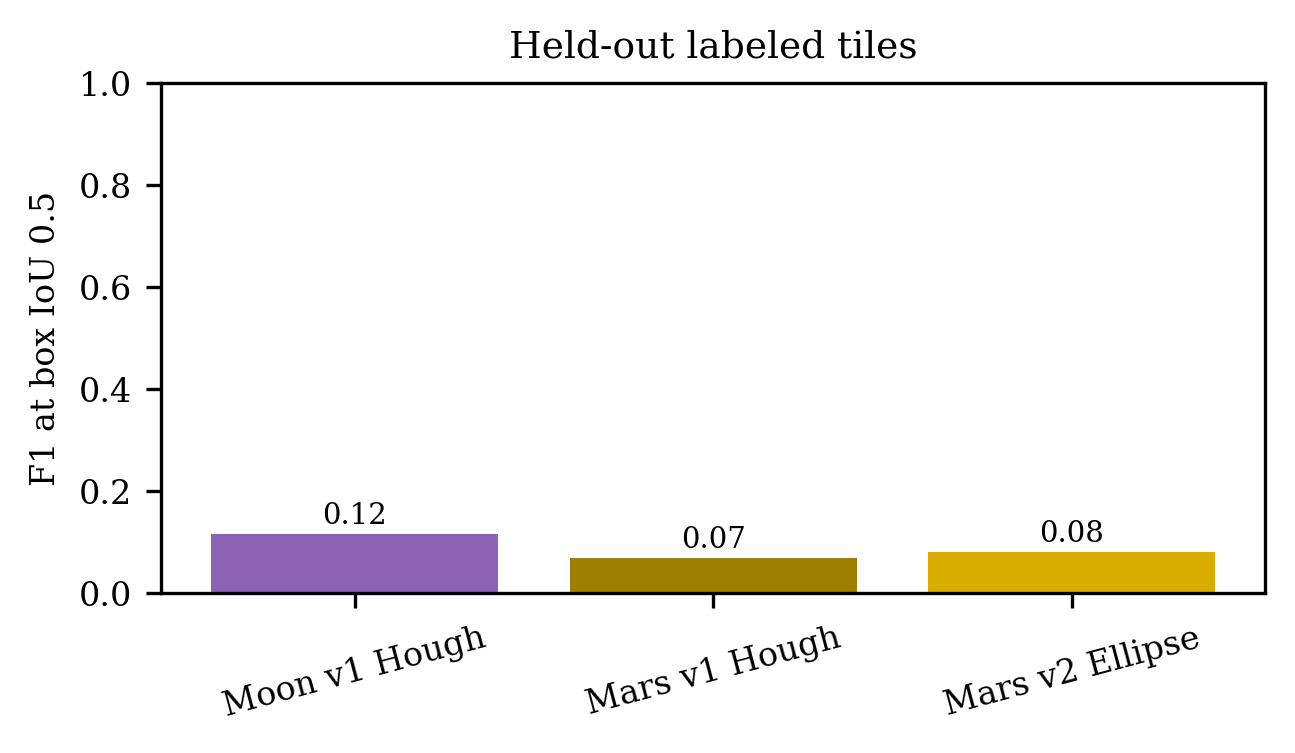
\includegraphics[width=\columnwidth]{validation_f1.png}
\caption{Held-out F1 by planet and detector at IoU 0.5.}
\label{fig:validation}
\end{figure}
\begin{figure*}[!t]
\centering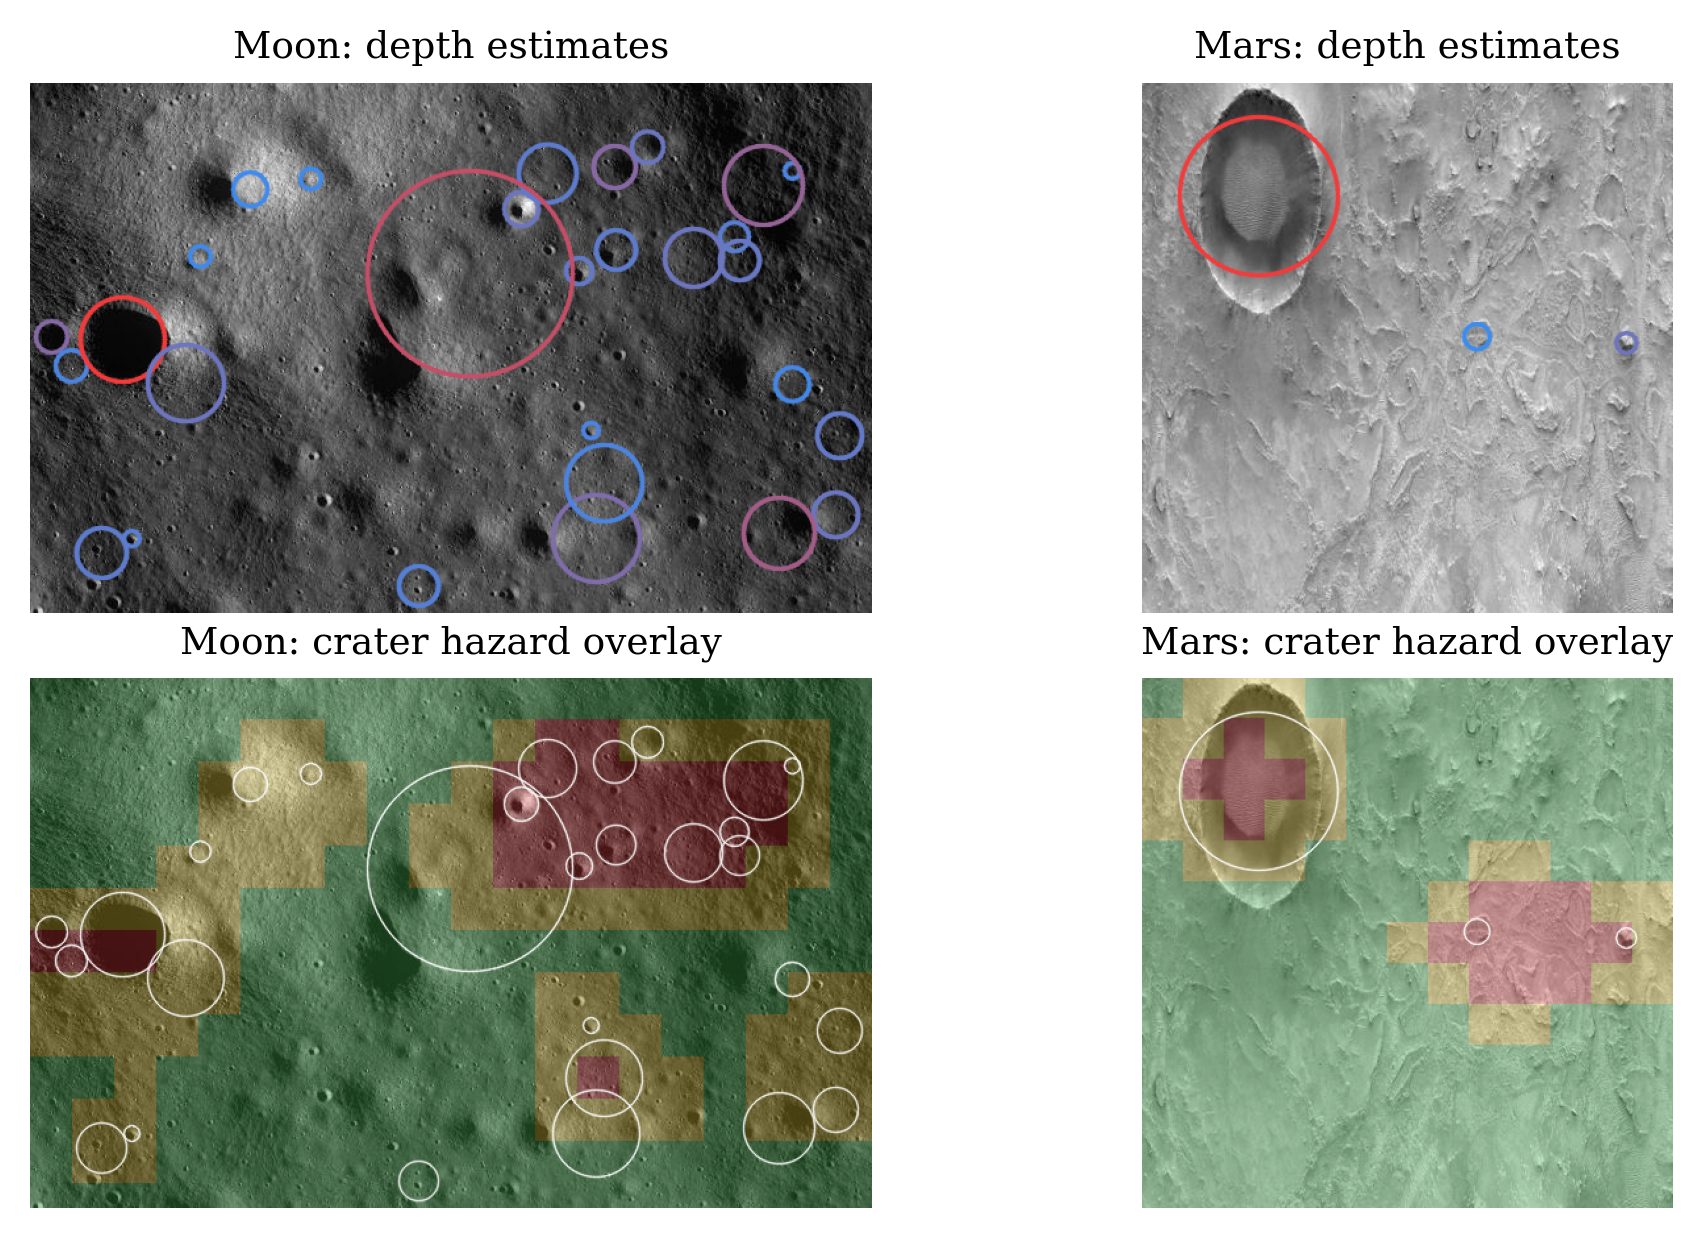
\includegraphics[width=.94\textwidth]{depth_hazard_maps.png}
\caption{Depth estimates and crater-only landing-hazard overlays from actual Moon and Mars tiles.}
\label{fig:depthhazard}
\end{figure*}

Fig.~\ref{fig:distributions} shows the size and degradation outputs. Mars meter-scale size classes use per-tile calibration when available and the configured fallback otherwise; the cross-planet diameter comparison is therefore not a controlled resolution comparison. No claim of comparable crater density is inferred from these tiles.
\begin{figure}[!t]
\centering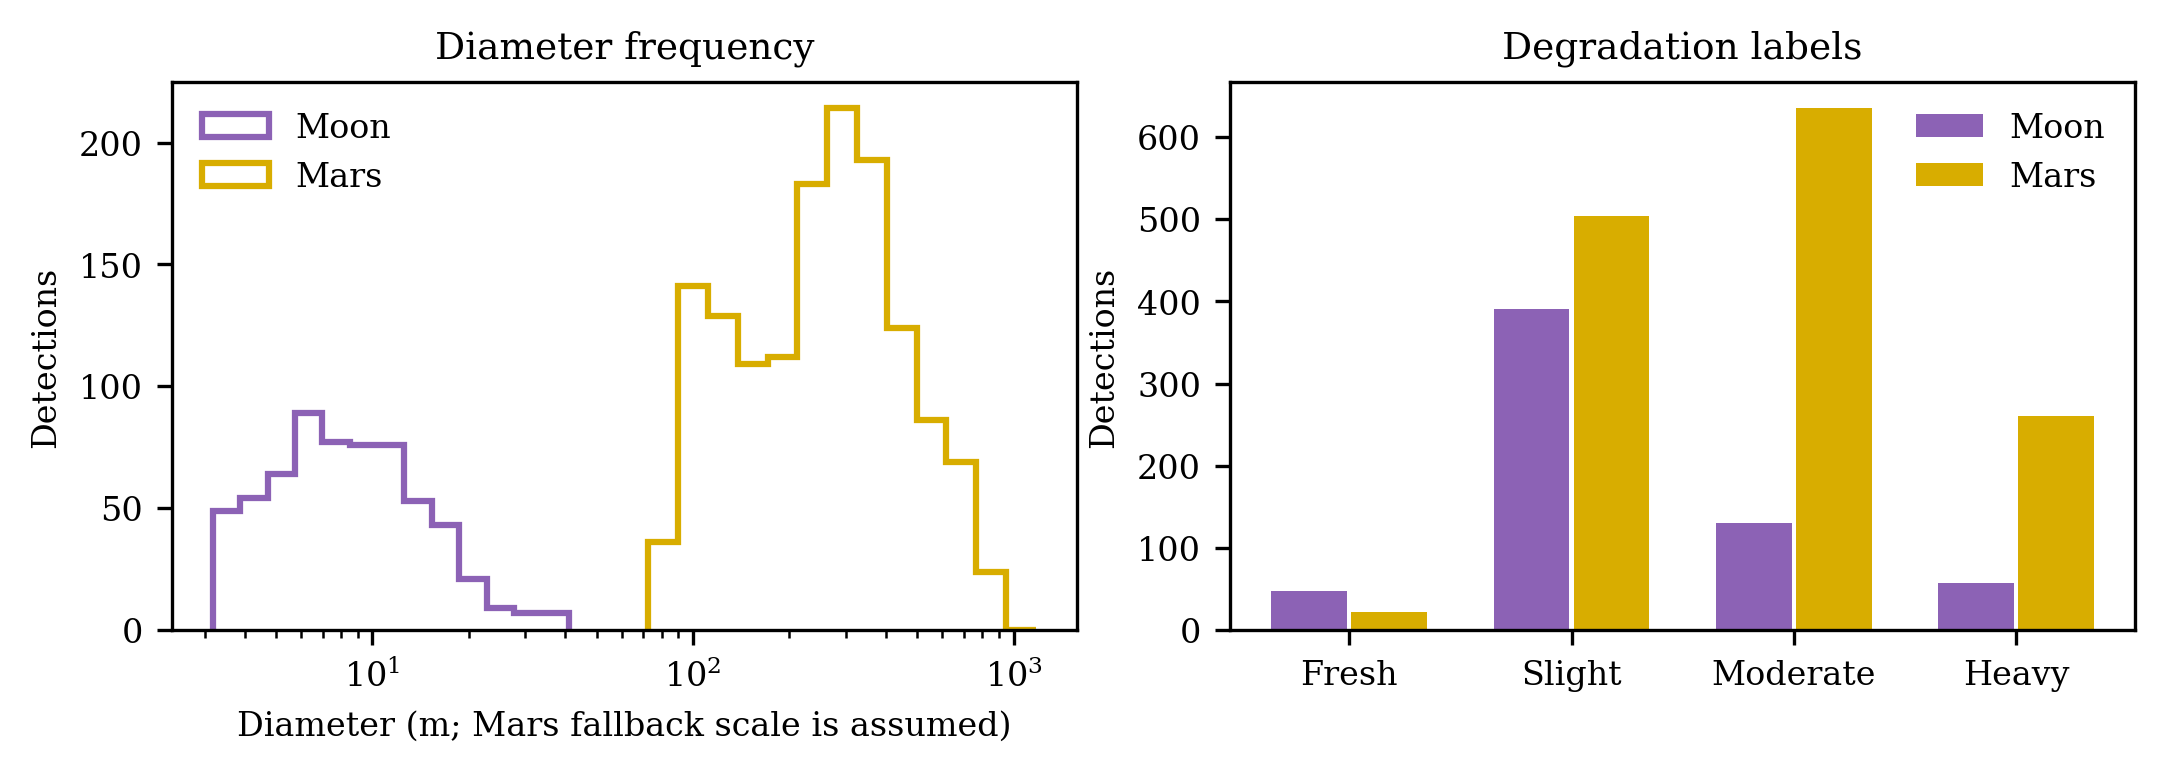
\includegraphics[width=\columnwidth]{size_degradation.png}
\caption{Observed detector diameter and degradation distributions. Mars scale is assumed for uncalibrated tiles.}
\label{fig:distributions}
\end{figure}

\begin{table*}[!t]
\caption{Mission-planner metrics for the selected example tile on each planet. The Mars scale is marked assumed when applicable.}
\label{tab:mission}
\centering\scriptsize
\begin{tabular}{lrrrrrr}
\toprule Planet & Landing clearance (m) & Path (m) & Straight (m) & Detour & Craters crossed (straight/route) & Min. rim clearance (m) \\
\midrule
\missionrows
\bottomrule
\end{tabular}
\vspace{1mm}\parbox{.95\textwidth}{\scriptsize * Mars route metrics use the configured fallback scale for this uncalibrated example tile.}
\end{table*}
The mission example uses the largest detected crater rim as the destination and the planner's balanced cost policy. The selected touchdown is the greatest-clearance candidate in the current crater-only map. Fig.~\ref{fig:mission} depicts the actual planner output; the red comparison segment is straight-line travel. Table~\ref{tab:mission} reports the corresponding metrics or a red TBD if a route is unavailable.

\begin{figure*}[!t]
\centering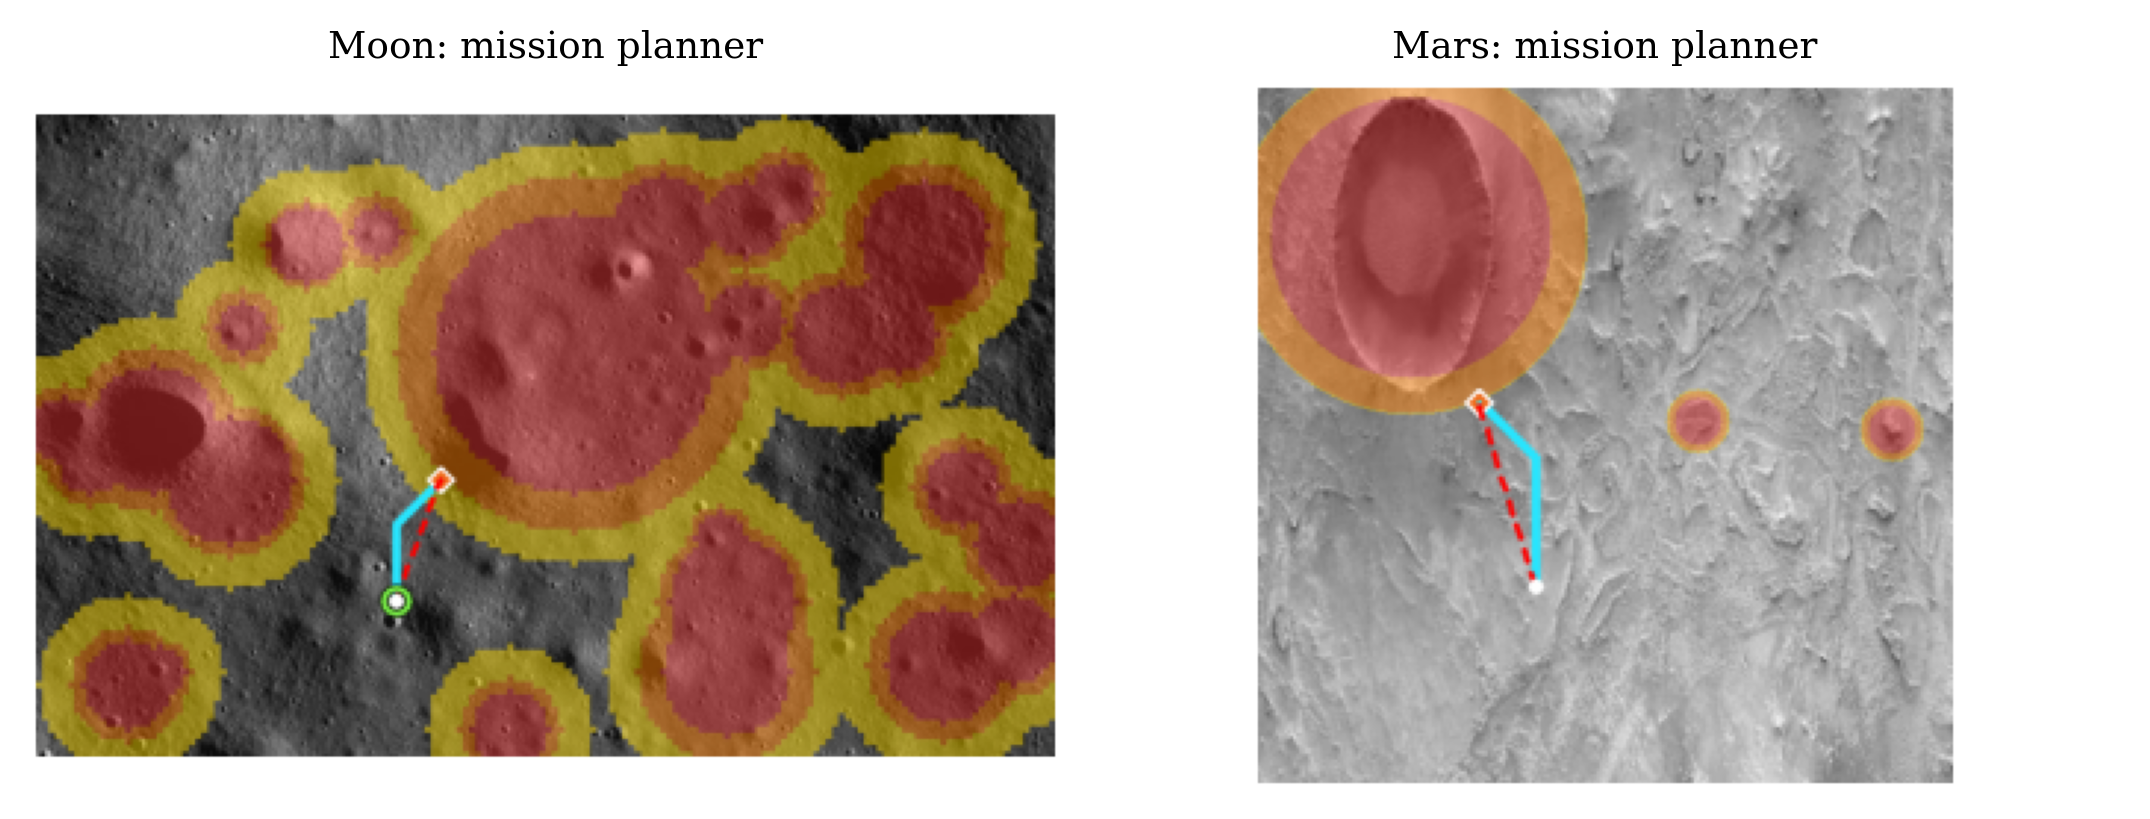
\includegraphics[width=.9\textwidth]{mission_planner.png}
\caption{Mission-planner outputs with touchdown, planned A* route, and straight-line comparison for actual example tiles.}
\label{fig:mission}
\end{figure*}

\section{Discussion and Limitations}
The principal result is a transparent chain from candidate image structure to an annotated measurement and an example navigation decision. The same visibility is also a limitation: local threshold choices and hand-set geometric rules remain exposed and can fail when rim contrast, illumination, or image style changes. Thresholds and detector defaults were tuned empirically. Hough circles fit elliptical craters poorly; the Mars ellipse fit still produces false positives and imperfect boundaries, as the box-matching results show.

The depth estimate is particularly fragile. It samples a single horizontal scanline and uses a relative intensity threshold; it does not measure a terrain profile or account for azimuth, surface albedo, photometric correction, or occlusion. Shaded/composited Mars images do not reliably encode cast shadows, so Mars depth and $d/D$ are low-confidence by default. Mars tile scales are per-tile when known but assumed otherwise; the dataset is mixed-source and includes imagery whose provenance and scale are not uniform. The lunar and Mars tiles are small samples, and densities are indicative rather than population estimates. Moon-vs-Mars comparison is only meaningful at comparable resolution and should use scale-free measures when scale is not comparable.

The planner's costs are an educational heuristic based only on detected crater geometry and a freshness proxy. It does not use slope, rocks, terrain elevation, soil bearing strength, illumination, vehicle dynamics, uncertainty-aware mapping, or onboard sensing. A missing crater detection can therefore make unsafe terrain appear traversable. The application states: ``Cost-map + A* search; uses craters only; real missions also use slope and rock data.'' Mission systems use richer terrain maps and sensing: the JPL Jezero hazard context includes safer and hazardous terrain and terrain-relative navigation~\cite{jplJezero}. This prototype should not be interpreted as flight-qualified site selection.

\section{Conclusion and Future Work}
This paper documented a two-planet classical-vision application that combines crater candidates, interpretable image-derived descriptors, hazard visualization, and a crater-cost A* route planner. The current exported runs provide a reproducible baseline, not evidence of operational accuracy. Future work should prioritize scale- and source-controlled labeled data, independent expert annotations, detector calibration by image domain, terrain-model-based depth validation, and planner inputs for slope and rocks. A quantitative uncertainty model and route validation against richer terrain maps would be needed before mission-use claims.

\section*{Acknowledgment}
The authors acknowledge [Acknowledgment placeholder].

\bibliographystyle{IEEEtran}
\bibliography{refs}
\end{document}
